\documentclass{my_paper}
\usepackage{ctex}
\usepackage[textwidth=444bp,vmargin=2.5cm]{geometry}%设置页边距
\usepackage{array} %主要是增加列样式选项
\usepackage[dvipsnames]{xcolor}%颜色宏包
\usepackage{graphicx}%图片宏包
\usepackage{amsmath}%公式宏包
\usepackage{enumerate}
\usepackage[T1]{fontenc}    
\usepackage{newtxtext, newtxmath}  %两种使用Times New Roman 字体的方法
\usepackage{listings}

\usepackage{paralist}
\let\itemize\compactitem
\let\enditemize\endcompactitem
\let\enumerate\compactenum
\let\endenumerate\endcompactenum
\let\description\compactdesc
\let\enddescription\endcompactdesc %解决Itemize和Enumerate的item之间行距过大

\usepackage{float}
%强制放置图片

\title{给数学系22级学弟学妹的一封信}
\author{Jay }
\date{\today}

%生成pdf文件的左侧目录
\usepackage{hyperref}

\hypersetup{
colorlinks=true,
linkcolor=black
}
%取消红方框

\begin{document}

\maketitle
\thispagestyle{empty}
%将目录页的页脚设置为空。

\newpage

\begin{center}
	\textbf{\LARGE 前言}
\end{center}

在19年刚入学时,笔者对大学生活一无所知,甚至没有咨询过学长学姐。自然,在很多地方上受挫,也有一些不可挽回的遗憾。诚然,福师大的校园生活一类的已经有太多人写过了,像数学专业学习你在知乎上也会找到各式各样的。尽管如此,像中科大他们数学专业学习进度、选课方法等等,我们并没有办法参照那种学习进度去原班照抄。

在20年,笔者在github上看到了\href{https://survivesjtu.gitbook.io/survivesjtumanual/}{《上海交通大学生存手册》},看到了不同人对如何过大学生活的不同观点。大学不会告诉你答案是唯一的,每个人都有每个人的路要走,录取师范类专业不一定代表你未来一定就想当老师,只有你自己才能决定自己现在做什么、将来做什么。

笔者只能基于自己当前的经历,尽可能的对数学专业学习做一下介绍。由于眼界限制,尚未接触到当下的就业行情、如何出国等等,自然没有办法写自己不熟悉的东西。

笔者衷心希望各位读者刚入大学时了解这些必要的知识能少走一些弯路。至于个人追求,这一点因人而异。希望各位读者能够有勇气、有智慧,去发现并找到自己所追求所向往的东西,尽可能不被外界所限制。

本文当前版本是使用overleaf进行\LaTeX{}编写的。如果您对本文内容有任何问题、或建议,请联络我们。本文主要来自20级蔡希晨(qq1005747513)和21级施可心(qq483970979) 。大家有问题可以私聊我们,内容不足之处请指正。

\begin{flushright}
	Jay \\
	\today
\end{flushright}




\newpage


\tableofcontents

\thispagestyle{empty}
\newpage

\setcounter{page}{1}
\section{专业分班篇}

首先欢迎大家加入数学系的大家庭,下面主要给大家解答下数学专业分班问题:

关于数学实验班(20级):

在新生入学后第一星期内,新生自愿报名参加实验班\textcolor[rgb]{1,0,0}{笔试}(大概报了80多个),其中前40名直接免面试录取,20个参加面试其中选10个(大致面试内容为:主要问你为什么进实验班,对研究生的了解,还要参考你高考数学成绩,英语成绩,还有一些灵活性的问题),合计选出50个组成实验班,其余人员按学号分到数本一班、数本二班

\textcolor[rgb]{1,0,0}{若想为开学后的第一次分班考做准备,由于20级考的大多是竞赛知识,所以建议做做中学生数学竞赛的题目;由21级考的题型只有填空和大题,填空类似高考填空最后两道,大题也与高考题型相似,但会有一两题拓展。比如21级就考了关于虚数的内容。}

大一上学期结束,实验班第一次重组,根据期末解几、高代I、数分I成绩(同分的情况下参考总绩点及外语成绩),从原实验班与数一、数二新报名的同学中再选出40人,前30名直接免面试录取,20人参加面试。原实验班退出20人。

大一下学期结束,实验班第二次也是最后一次重组确认人员,共选出30人组成实验班。但是听说大三因为政策变革又改回实验班50人了。不知道别的年级什么情况。

关于数学实验班(21级): 

大一分班情况与20级相同。目前还是40人。


\subsection{个人建议}
在数一和数实各呆了半年然后现在还在数实的学长的建议:如果想过的相对轻松一些,多做一些自己想做的事,留在教师班挺好的。实验班作业量相较于教师班会大挺多(平均至少都要2.5小时吧,花一个晚自习时间有时也做不完,周一到周五晚自习6点半到9点),会牺牲掉很大部分可支配的时间。\textcolor[rgb]{1,0,0}{就保研名额分配、评优评先等,在改革后是三个班合起来评的。}

在大一、大二阶段,教师班与实验班所有课程设置上\textcolor[rgb]{1,0,0}{没有任何区别}。除了大三的部分专业选修课不同外,整个专业都是按\textcolor[rgb]{1,0,0}{数学师范}来培养的。所以不存在实验班教的教学技能可能比教师班少这件事。大一阶段的区别,老师在实验班会多补充一些课外知识。比如如果课本的讲法不是很好,他就会换一本书参考着讲。

你只要考虑好自己大一是想花很多时间在数学上还是其他地方上就够了(比如社团、活动),大一上结束我们常常会发现近一半同学就退出实验班:一部分是报名之前根本就没想清楚自己是否能花那么多时间在数学专业课上,这并不比高中轻松。

当然也可以考虑去不同的班级呆一学期,体验一下不同老师的授课风格以及学习氛围。数实原则上是要读研的。如果后期有读研打算,在实验班可以听到挺多课本以外的拓展知识,对之后还是有好处的。

当然如果你想学的更深刻的一点,或者对自己的方向不太明朗,我建议你不妨跟不同的老师聊聊天。

强烈建议大家也可以稍微想一下\textcolor[rgb]{1,0,0}{自我介绍},刚开学,同学相互都不认识,很经常需要让大家进行自我介绍。更不用说面试一些部门和岗位。提前准备四五句话,这样到时候就不慌啦。

\section{社团与学生工作篇}
简单聊几句社团和学生工作。

刚来大学的时候,我们很可能都有一种错觉:认为自己什么都应该去做、去尝试。然而,一个人的精力是有限,我们中大部分人都不是那种全能型天才,各个方面都强到爆表。感兴趣的方面也并不会每个都做到很擅长。社团是一个很好的平台,你选一些自己感兴趣的,参加参加活动。学生工作更侧重于培养你和人打交道、处理事情的能力。

我始终认为适当的社交能力是必要的。至于什么是\textcolor[rgb]{1,0,0}{适当},这一点因人而异。

我个人的建议是选学生工作岗位时,\colorbox{-blue}{尽量问问学长学姐看看},也会有各个部门的扫楼宣传活动,\colorbox{-blue}{大家要清楚各个部门负责的活动和根据自己的喜好和能力选择适合的学生工作。}权衡自己擅长什么是一件很难的事,但你多去问一问,可能就会有不一样的想法。个人建议做一份学生工作,选择1-2个社团(学生工作、社团干事会忙一些)。

在社团、部门里,社员和干事是不一样的。学生工作大体划分的话,应该是班级、年级、院级、校级。至于详细说明你可以看看他们的宣传。
   
另外,数学系的同学可以考虑加一下数学教育协会,是数统院最大的社团,开展教师技能类以及学术知识,数学文化类活动,协会提供线上辅导,邀请成绩优秀的学长学姐在答疑群里给同学们解答问题,以及半期考辅导,进行往年的相关卷子讲评,协会还提供数学类以及高数类的往届考试资料,举办的教师技能大赛,中数竞赛,数学嘉年华等,大部分活动参加成功可以有参赛证明,加综测分。每次活动的参加可以累加协会时长,20个协会时长可以换取毕业需要的一个素拓分,开学会有扫楼,将有详细的介绍,可以在扫楼的时候关注一下,真的入股不亏,白嫖的复习资料,还可以认识到新朋友呀!

\section{学业篇}

\subsection{课程介绍}
出于高中与大学的衔接,你可能需要了解和熟悉的:数学归纳法、反证法、常见的放缩法等。因此我比较建议你看一看高等代数简明教程的\textcolor[rgb]{1,0,0}{引言}部分、谢惠民的数学分析习题课讲义的引论部分、梅加强的数学分析的引言部分。

首先要说的是:数学系课程难度还是挺大的,数分1第一学期期中考就挂了67.39$\%$,高代第二学期期中考挂了58.06$\%$。\textcolor[rgb]{1,0,0}{自学}是进入大学以后的第一门课程,学会自己查资料,选择一本自己适合的教材也是很重要的。

另外就是大学第一个课程特点就是:上课强度大、内容多。有的课因为课时原因,老师很可能也要赶教学进度。而复习、理解知识等等全靠自己自觉去做。像数学分析这种前后联系很密切的,落下几节课后面基本都听不懂了。

(具体课程介绍见\nameref{sug})

   \subsection{关于讨论班}\label{s}
(节选自楼红卫老师的数学分析注记,见\nameref{f5})

让学生尽早参与讨论班。讨论班是一种在数学界广为采用的培养研究生的主要模式,很多数学教师在高年级本科生的论文写作中也采用这一模式。讨论班主要\textcolor[rgb]{1,0,0}{由学生讲解}自己查找的或指导教师预先给定的论文或书籍,讲解过程中接受指导教师和同学的\textcolor[rgb]{1,0,0}{质询},质询过程中,指导老师和同学不仅可对讲解内容的正确性和某个结论的证明提出刨根问底式的询问,甚至还会就内容的选择是否恰当进行质询。在讨论班上,学生除了扮演学生的角色外,同时扮演了教师的角色。它迫使学生学得更深入、更透彻、更前沿。

    对于本科生而言,在低年级就引进讨论班机制,虽然不一定可以让学生走到学科的前沿,但在增强学生的学习深度等其他方面,取得的成效是明显的。一般说来,讨论班的规模不宜过大,以六人以下二人以上为宜。对于选题,指导教师除了提供大的学习/研究方向,在具体学习/研究材料的选取上,是否也由指导教师确定,要视具体情况而定。教师直接指定材料,容易让学生早日进入角色,成效的显现也比较快。但让学生自己选取材料,对培养学生独立的学习研究能力非常重要,发展的后劲也更大。如果能够长期坚持讨论班的学习模式,则应该设置让学生自己选取讲解材料的环节。
    
20级大一阶段汇报的材料的谢惠民的习题课讲义,以及自选的复旦高等代数习题课、每周一题。

21级大一阶段汇报的,除20级用的,还有裴礼文的《数学分析中的典型例题与方法》和一些数学竞赛试卷的题目。

有兴趣的同学可以先\textcolor[rgb]{1,0,0}{组织一个小组}试一试,至于讨论班的内容选取、场地等等问题,你可以咨询一下老师。

大一阶段还是要多做一些题,但不是盲目去做,多总结多思考解题方法,以此来建构整个属于自己的知识框架。注意,做题只是强化你对知识的理解,通常可能有这几个阶段:
\begin{itemize}
    \item 通过各种渠道(包括网课、其他书籍)看懂课本说的是什么,往往很多时候有些大学课本并不会告诉你问题背景。
    \item 忘了课本前面讲了什么,因此才要做一些题目理解这些定理、命题在哪些方面可以用到。
    \item 总结和思考。合上课本自己构建整本书的知识体系。
\end{itemize}


\subsection{关于绩点、学分、综测}

\subsection{关于竞赛}
数学系主要的竞赛还是数学建模和数学竞赛。
\subsubsection{数学建模}
数学建模由三个人组成,建议是两个数学系的带上一个软工或者计本的(找个会用python或matlab画图的就行,专业不限)。虽然说三个人位置可能是分开的建模手、论文手、编码手,但一定都要懂得队友位置的工作在做什么。(每个人都要会写论文)

也就是不但要各司其职,更要在必要的时候协助队友工作。

至于建模经验帖网上有很多,这里就不加赘述了。有兴趣的同学可以到b站或知乎找找。你想要数学建模准备充分是不大现实的,只能以赛代练。每一次建模经验其实对你和你的队友来说都是弥足珍贵的。
\subsubsection{数学竞赛}
数学竞赛的话比较硬核,学数分高代的时候就要扎实的学,并多次翻回前面复习。老老实实把习题课讲义和高代白皮书理解透了,我个人认为差不多够了。

由于全国大学生数学竞赛近几年都在11月中旬,所以只有大二及以上才能报名参加,当然在每年的5或者6月,也有校数学竞赛,你可以好好准备一下校赛小试牛刀。

我们如果是打国赛的话属于最难的数学专业A组,去年甚至考了一下比较偏的、有偏微分背景的问题。个人建议:不要因此而太着急学后续课程!!老老实实把数分高代一些繁琐的证明做了!!主要是你急着学了后面的东西,你不知道前面知识的背景等于白学。(就好像你看A和B拳击比赛,你知道A赢了只学A的招式,然而你不知道A是为了针对B而研究的招式。所以我建议有可能的话还是\textcolor[rgb]{1,0,0}{多了解知识背景})

所以还是把握好自己能拿到的分!!\textcolor[rgb]{1,0,0}{好好学解几,解几这几年都相对简单,如果解几没拿到分,基本都很难拿奖。}
大学生数学竞赛考察内容:数学分析、高等代数、解析几何(所占总分的比例分别为50$\%$、35$\%$、15$\%$)。

其实数学也是一种类似于学习语言的过程;解题步骤应模仿例题的语言,使自己的语言尽可能变得规范严谨。(想想大家以后也是要当老师的嘛,养成好的习惯,采用的数学语言和课本一致,学生才学的清楚)

\subsection{关于英语}
从19级开始,大一上是可以考四级的(在12月中旬,四级词汇量可能比高考多一点)。必须过了四级才能考六级。保研名单基本上都是通过了四级和六级的。但是六级相较于四级难度差挺多的,要多花时间准备。

英语一级班和二级班的区别:二级班免修大英一,即大二下没有英语课。
建议:至少四级考个550在大二上选免修,580免修血赚。

20级:直接按高考英语分数分班。

21级:直接按高考英语分数是否上120来分班。四级540免修。
期末考出的有一半是U校园的听力、阅读原题,还有书本上会划重点。

\begin{figure}[H]
	\centering
	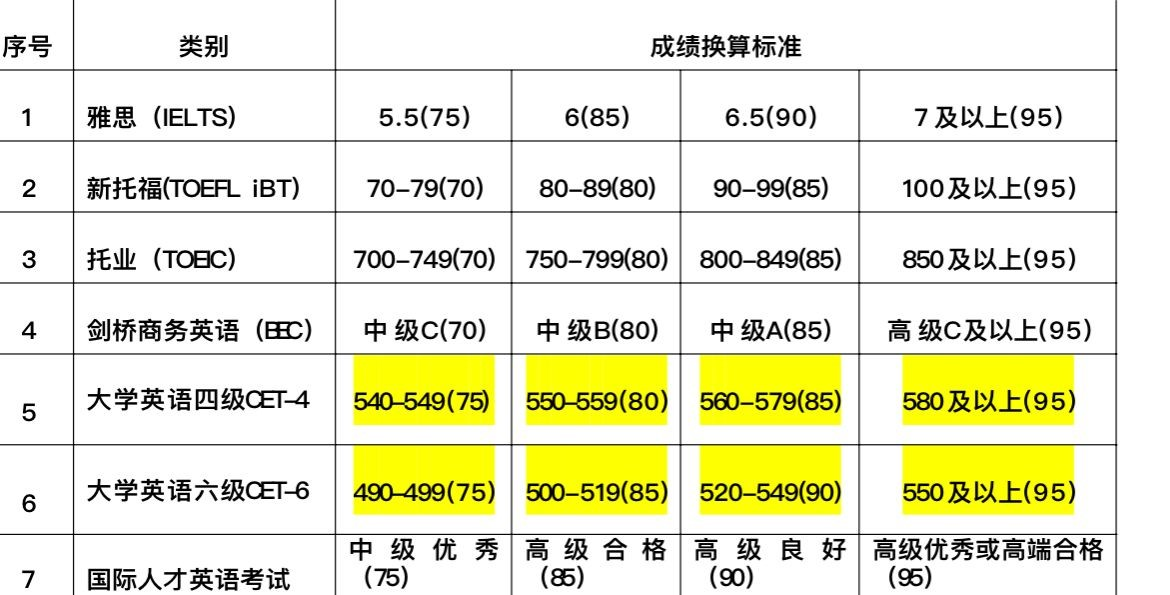
\includegraphics[width=0.75\textwidth]{English.jpg}
	\caption{分数换算规则}
\end{figure} 

请最好有意识的去养成自觉每天学一点点英语的习惯。你身边可能会有很多人不自觉,即便我也很容易这样。

\section{关于军训}
21级军训时间为12月5日到12月16日,12月的军训总是会比9月份好很多的。

先介绍一下军训流程

军训前一天会让大家去领军训的衣服,收拾好宿舍。军训地点为东区、西区、南区田径场(具体等学校通知),所有学生按学号分在一连,二连,三连以及后勤部。后勤部主要由因为身体等原因不能参加军训的同学组成。军训第一天会给每一个连分配一个教官,之后的训练项目有分列式、军体拳、包扎、踢正步、唱军歌等,最后一天是汇报演出和考核。所有的考核成绩将记录在学院的总分里。

军训的一个非常麻烦的重头戏就是内务整理,宿舍要收拾的跟没人住的一样,我在最后会附一张内务整理标准。等大家军训的时候辅导员也会时时刻刻强调内务整理的重要性的。

训练时间:早上七点五十集合,十一点半前结束;下午一点四十集合;五点半前结束;晚上唱军歌;(因为隔得有点久,所以具体时间我有点模糊了,但基本上是这样)。

军训前几天教官会让大家学习走分列式(就是走个整齐度、走出精气神)以及踢正步,之后,教官会挑选出走的比较好的同学组成一个分列式队伍单独训练。这里强烈建议大家在教官选的时候好好表现,我之前也是觉得去走分列式会很辛苦,但去了以后是真香。因为接下来每天我们都只要走分列式和踢正步,而其他同学则要学军体拳、包扎等,并且最后会考试考这些内容。而我们全不用,除了腿酸以外基本没有任何坏处,而且相较来说也没有那么辛苦。

但是呢,没有进分列式的同学也不要惋惜,掌握一套军体拳就是防身多一份技能。唱军歌一般是在晚上,会请音乐学院的学长学姐来教,一定要互相尊重。每年军训唱军歌都会有很多花样,等到时候你们自己体会吧!最后一天会有一个战术表演,但基本上都是由体育学院的同学来表演,十分精彩。

会遇见不同风格的教官,大家敬请期待。

具体的注意事项等大家军训的时候辅导员都会通知大家,我就说一些我觉得要注意的点:
\begin{enumerate}
    \item 一定要有集体荣誉感,虽然军训只是每个大学必备的形式,但是希望大家可以在这段时间学会处理好个人利益与集体利益的关系。终身受益。
    \item 12月的太阳依然很晒,无论男生女生都要做好防晒哦,不要中暑了。一定一定一定要做好防晒,千万不要怕防晒霜涂多了,太阳可是很毒辣的。
    \item 所有训练项目都要量力而行,有不舒服要及时报告教官不要不好意思。
    \item 军训期间可以把刷手机的时间拿去刷U校园和一些学习通的公共课网课,十分有效
    \item 多吃饭多睡觉
    \item 大部分训练的枯燥无味需要大家有一个好的心态去克服。
    \item 走分列式的同学尽量当个前面举旗的,大概率会被评为优秀学员。
    \item 没事就不要不参加军训,不然第二年还是要补的。
    \item 勇于尝试,军训期间还会教枪的使用,由于每个排的枪支数量有限,教官通常只进行演示,不会统一教学,所以一些想要体验的同学要勇于抓住机会,教官人很好的,会同意一对一教学。如果想拍照留念的话可以找采编部的小伙伴,用相机拍下来。
    \item 休息的时候会进行才艺展示,所以多才多艺的你们可以提前准备哦,不要吝啬展现自己,军训是一个很好认识同学的时机,也是一个让大家认识你的好时机。
    \item 军训期间脚会很酸,可以拿运动鞋的鞋垫垫在军训鞋里,晚上泡泡脚,这样能有效缓解疲劳。
    \item 大家一定要积极参与哦,这样整个军训期间下来,就会发现其实还是有很多美好的回忆的。
\end{enumerate}


\section{关于个人规划}
\begin{figure}[htbp]
	\centering
	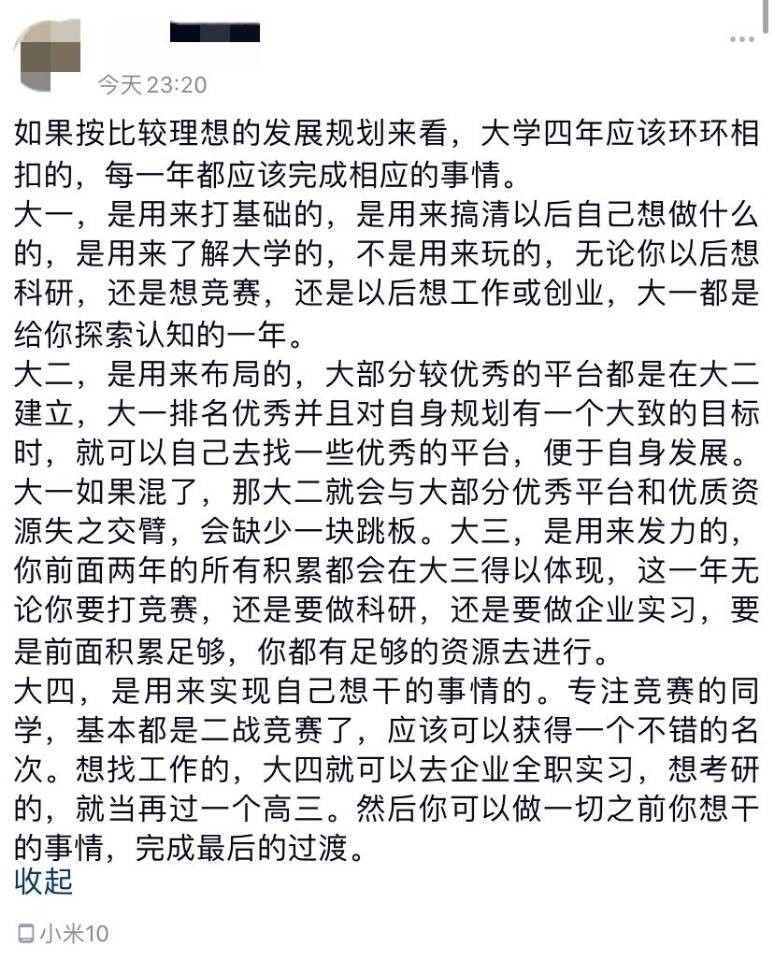
\includegraphics[width=0.8\textwidth]{gh1.jpg}
\end{figure} 

\begin{figure}[htbp]
	\centering
	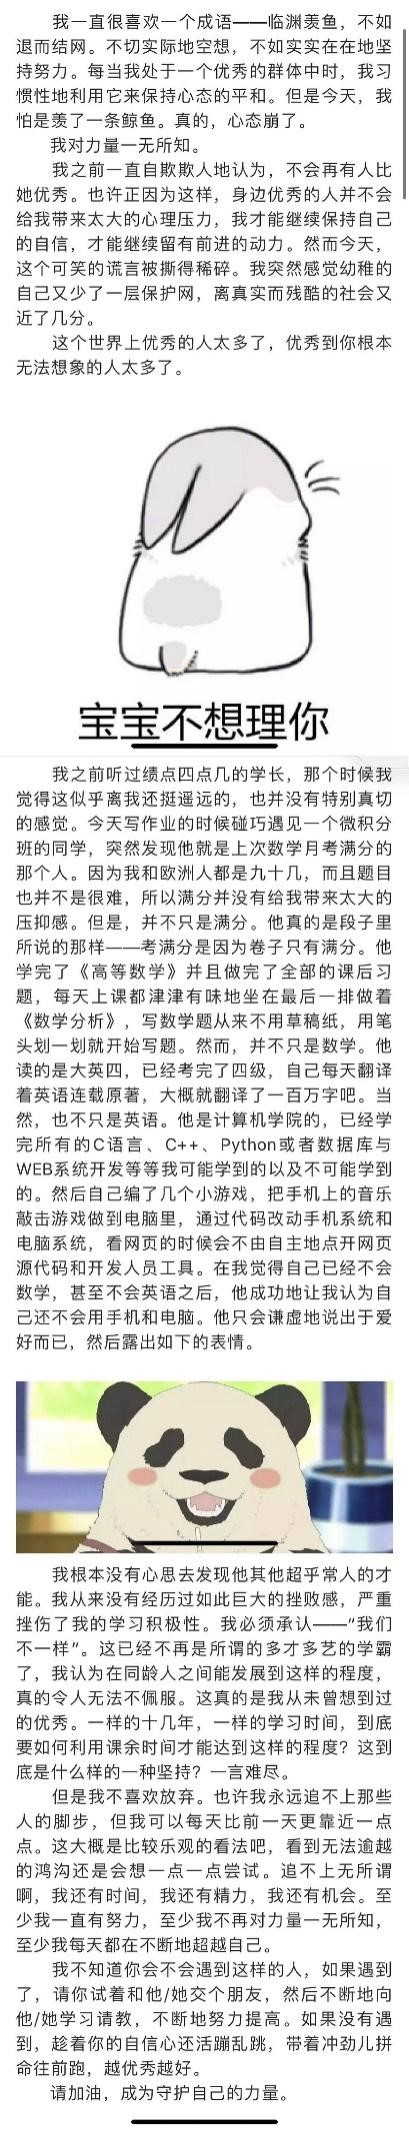
\includegraphics[width=0.3\textwidth]{gh2.jpg}
\end{figure} 

\begin{figure}[htbp]
	\centering
	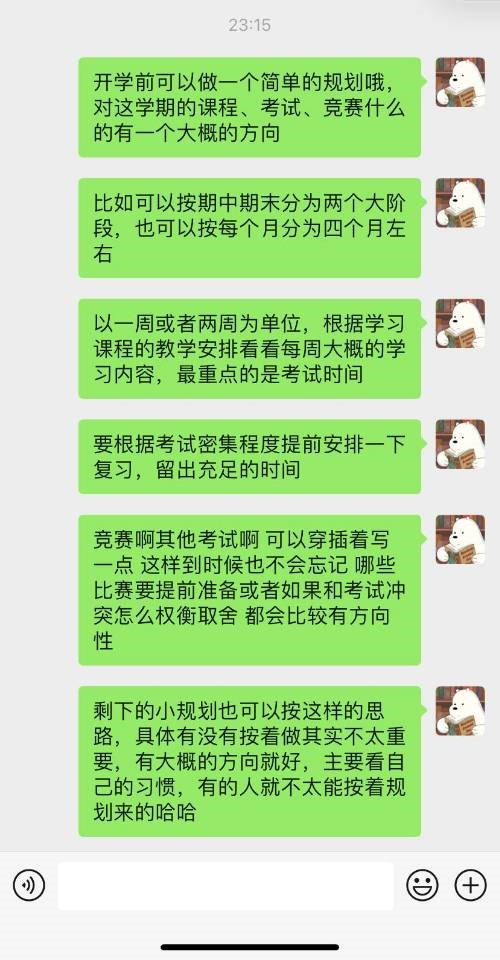
\includegraphics[width=0.8\textwidth]{gh3.jpg}
\end{figure} 

\newpage

\section{大一寒暑假安排的建议}
建议不要虚度大学的每个假期吧;假期有很自由、可自我支配的时间,这相较于在学校有的时候,我个人感觉每天要接受新的概念、复习、交作业而疲于奔命。假期有很充裕的休息时间,可以看自己想看的书而不受到上课时间的约束。

假期并不像想象中那么长,建议可以比如安排每天复习课本一小节的内容。学习是一个有加速度的事情,或者说也需要保持一定的手感。我目前逐渐习惯每天要做一定量的数学题,学一定量的新东西。虽然遗忘是一件不可避免的事情,所以有的题目很可能要做了,忘了,再做一遍。

根据个人学习习惯合理安排新知识和做题的分配。学新知识一定要主动去做题。我个人感觉数分跟着老师进度更舒服一些,所以一直没有提前学,只是参考别的教材补充内容。

有兴趣看书可以参考别的教材的讲法以及网课,不要太急着看后续课程。准备竞赛的建议大一上寒假刷完大一上对应部分的谢惠民、白皮书,遇到不会的题目多跟同学们聊聊,实在做不出来问问老师、助教,或者看知乎、b站、微信公众号上也有别人数分高代打卡。

\section{一些碎碎念}
最后,说实话数学系的孩子是很苦的,他们没有什么时间娱乐。我觉得数学做到后面不是靠天赋,而是靠信念和坚持。不要和别人比。希望大家把大部分时间用于专业课的学习中,认真细心扎实的学,最后一定会有收获。学习不要太功利,做到成功不骄傲,失败不气馁,时时刻刻保持谦逊才是学者风范。人生中能让我们好好学习的时间也不多。时常关注自己的状态,注意劳逸结合。

我们不仅要在大学学习知识,更重要的是学会做人。努力学习之外也要记得享受生活,如果一些社团活动有特别感兴趣的,你觉得有意义就去参加吧!希望大家能够用好大学这个平台,听从你心,学你想学。

\section{附件}
\subsection{附件1:大一下实验班考核依据}\label{f1}
考核依据为:第一学期英语课成绩不及格者直接退出选拨,其余同学计算第一学期专业课成绩(解几、高代I、数分I)的平均标准分并排序, 

注:各科标准分 Zi=(原始分-平均分)/标准差, 

三科专业课平均标准分=$(\sum_{i=1}^{3}(300+100*Zi))/3$,

其中Zi(i=1,2,3)为3科专业课的标准分。

(1)平均标准分在前30名的直接入选;
   
(2)平均标准分在第31名至第50名的参加面试,根据平均标准分和面试成绩总和排序,成绩前10名的同学入选。

注:相同得分的情况下参考总绩点及外语成绩。

\newpage

\subsection{附件2:22级数本各班课表}

\begin{figure}[H]
	\centering
	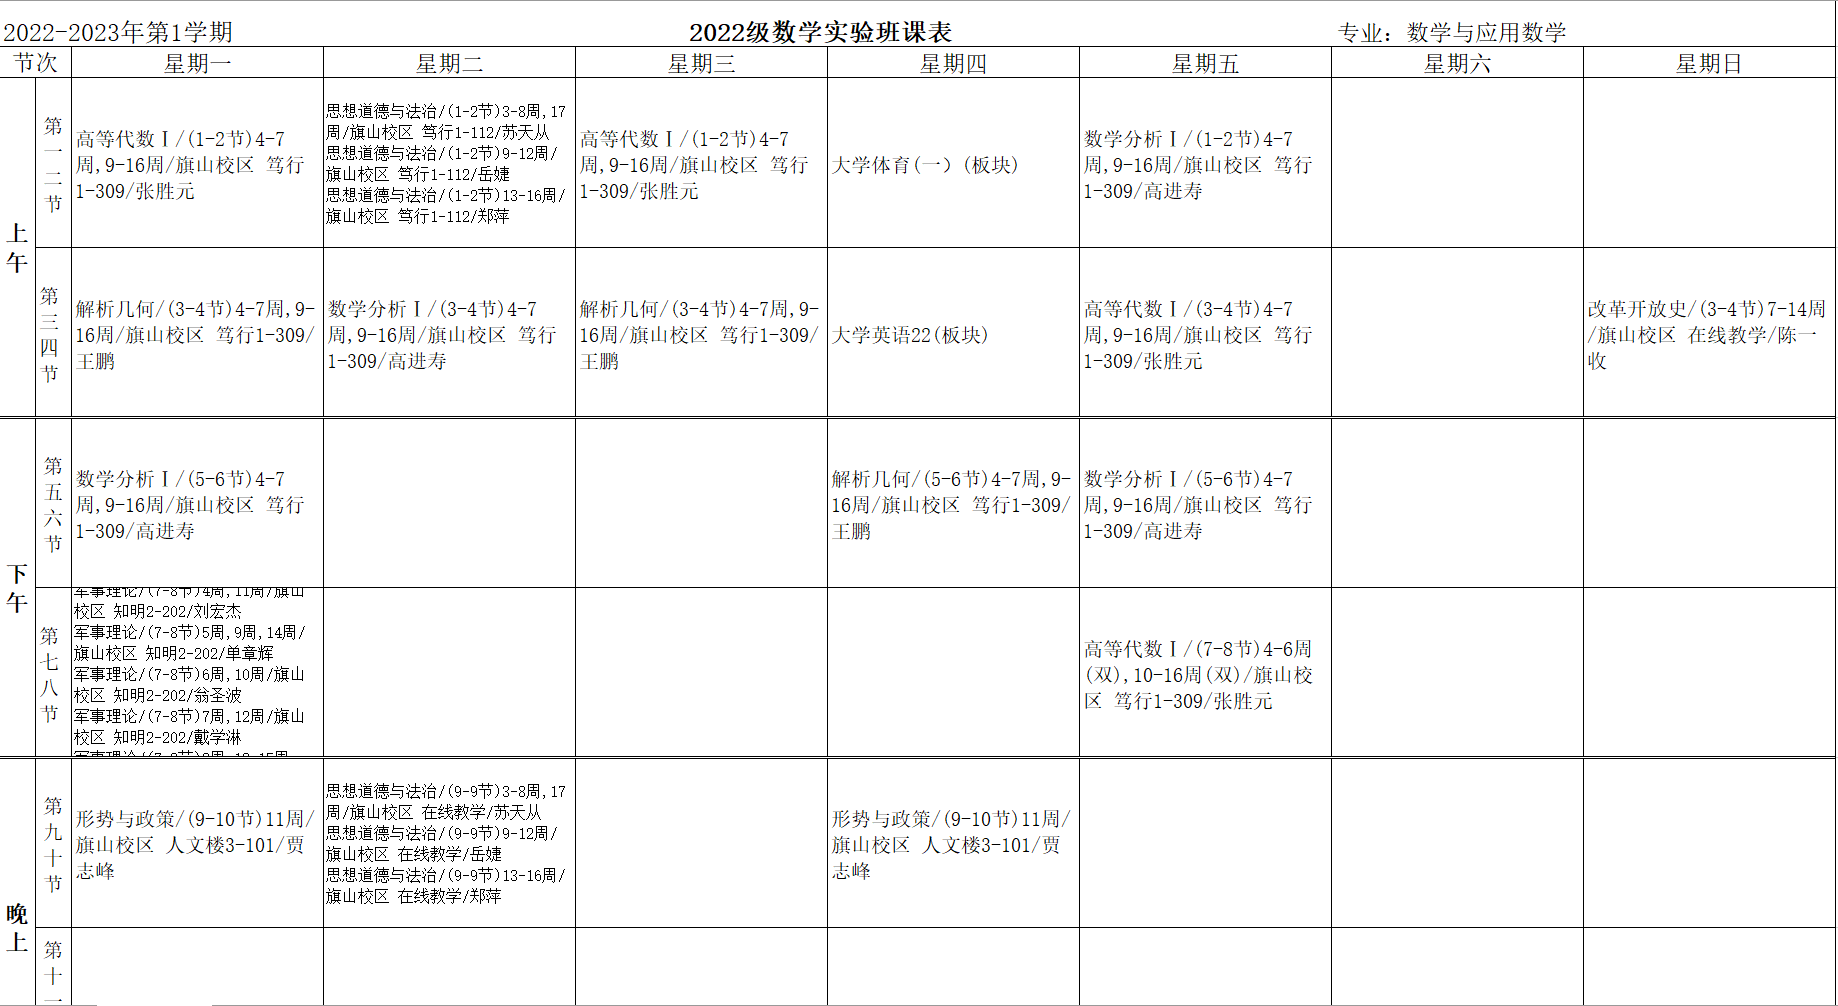
\includegraphics[width=0.9\textwidth]{实验班.png}
	\caption{实验班课表}
\end{figure} 

\begin{figure}[H]
	\centering
	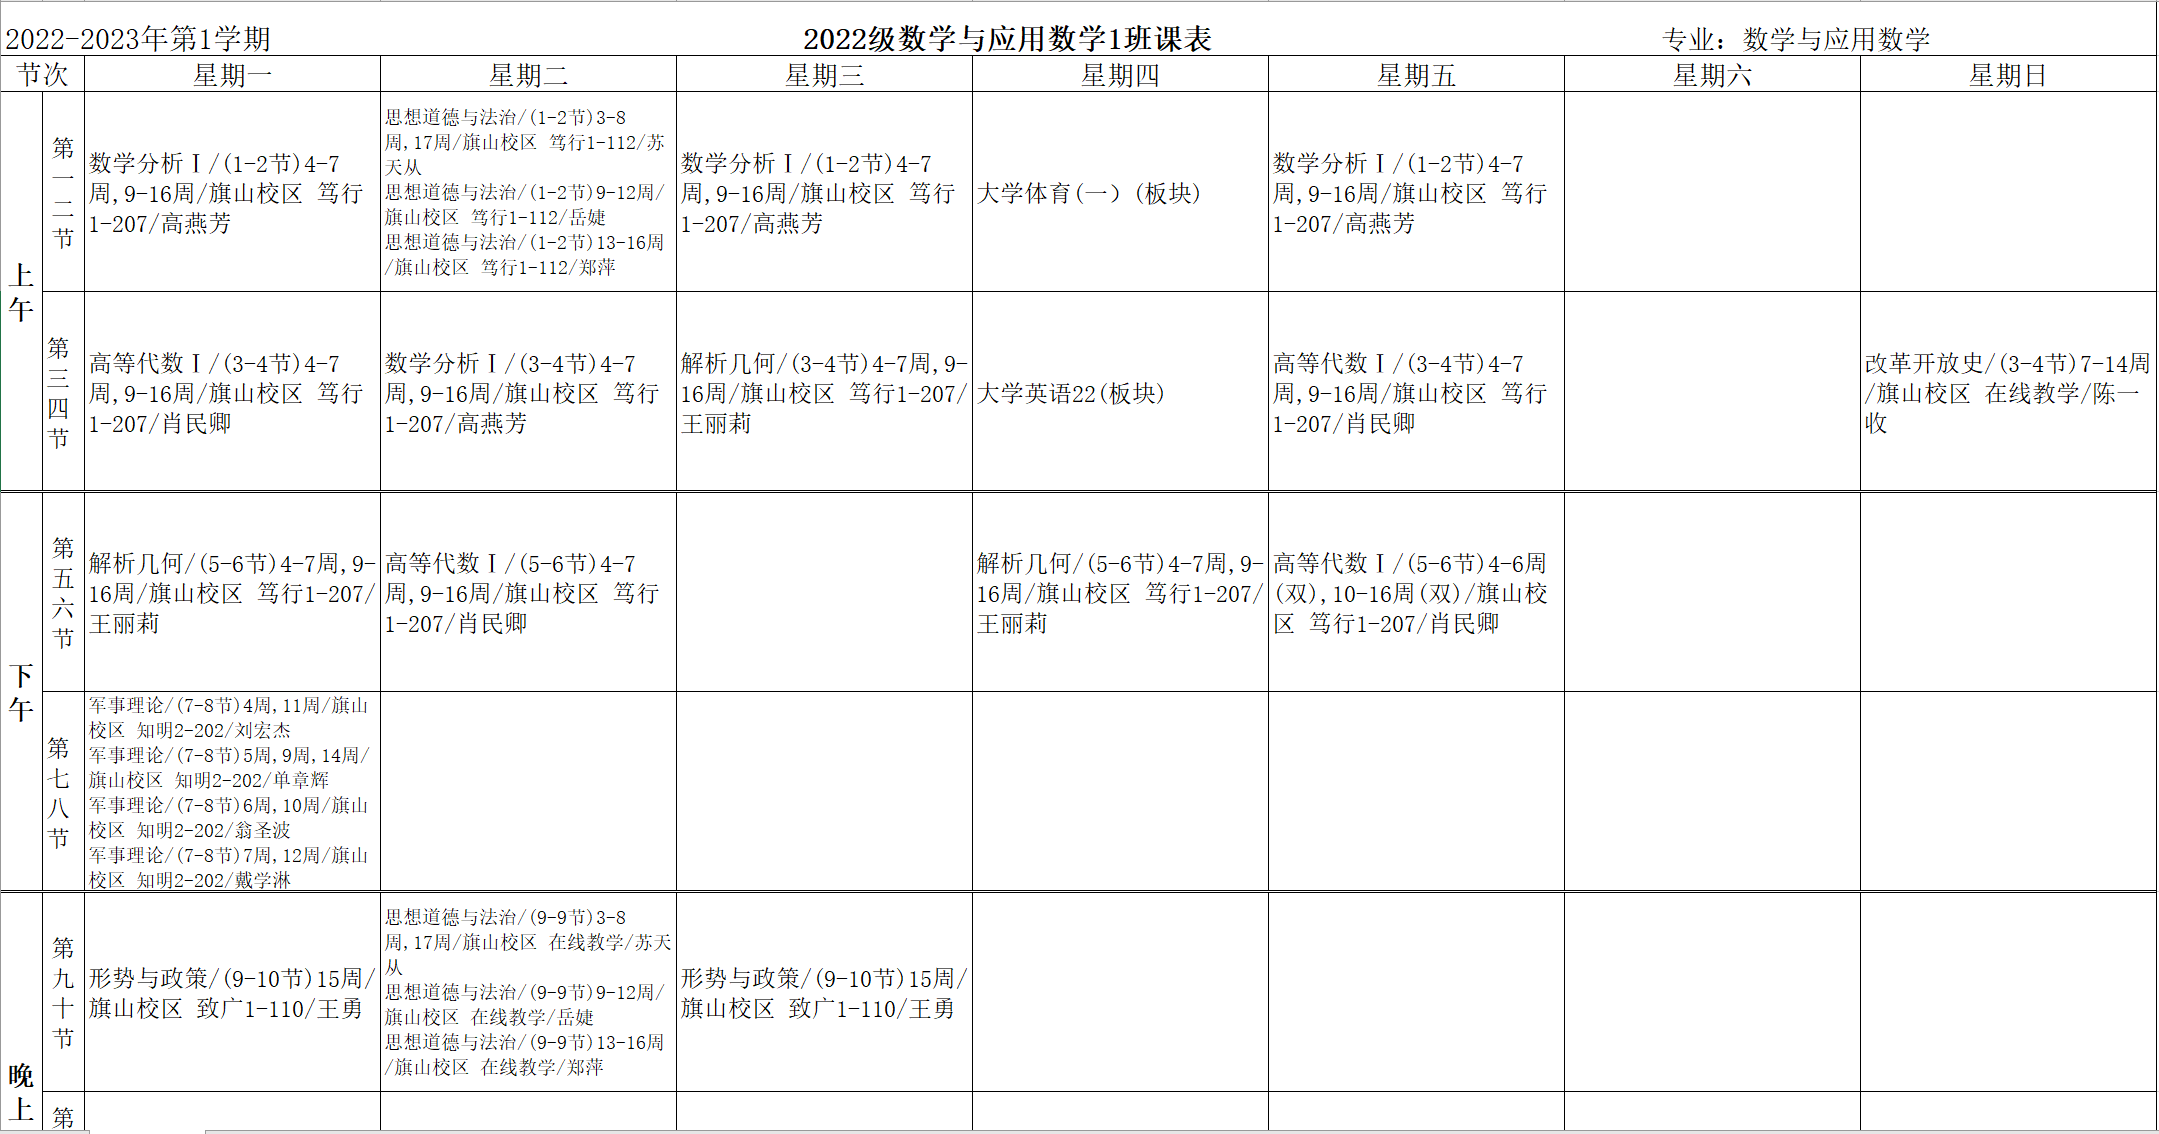
\includegraphics[width=0.9\textwidth]{数一.png}
	\caption{数本一班课表}
\end{figure} 

\begin{figure}[htbp]
	\centering
	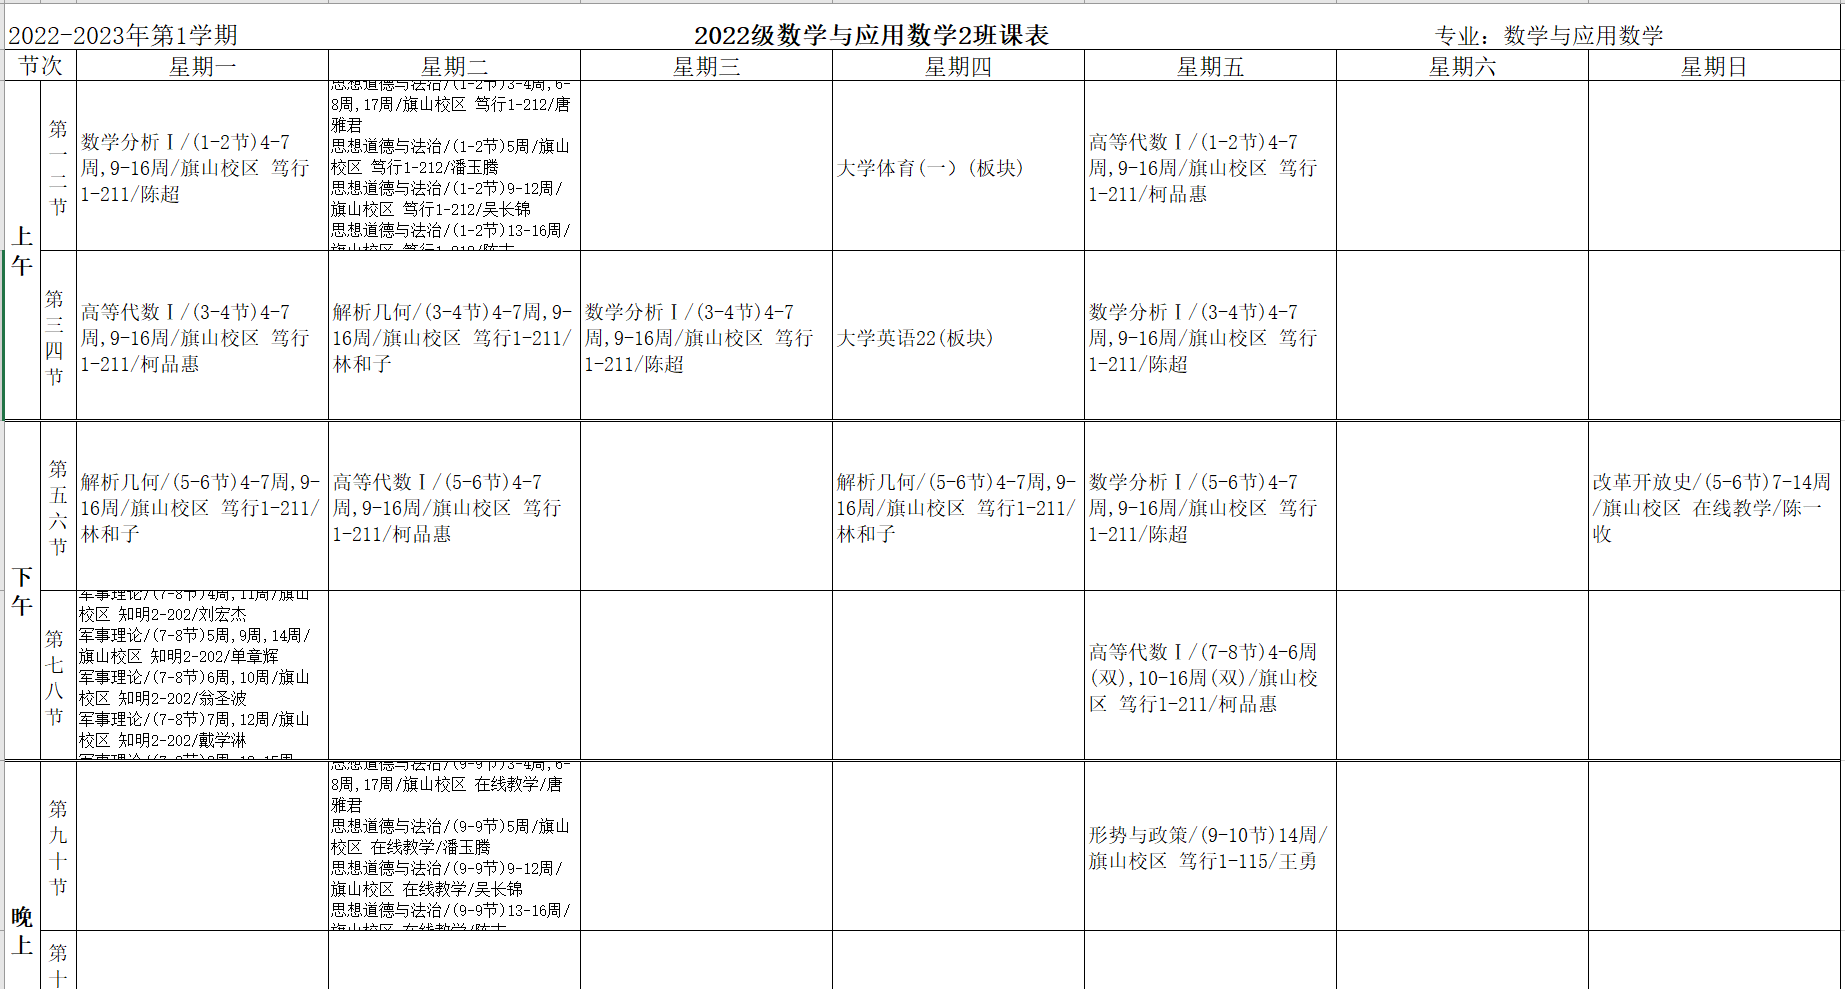
\includegraphics[width=0.9\textwidth]{数二.png}
	\caption{数本二班课表}
\end{figure}

\newpage

\subsection{附件3:作息时间}
\begin{figure}[H]
	\centering
	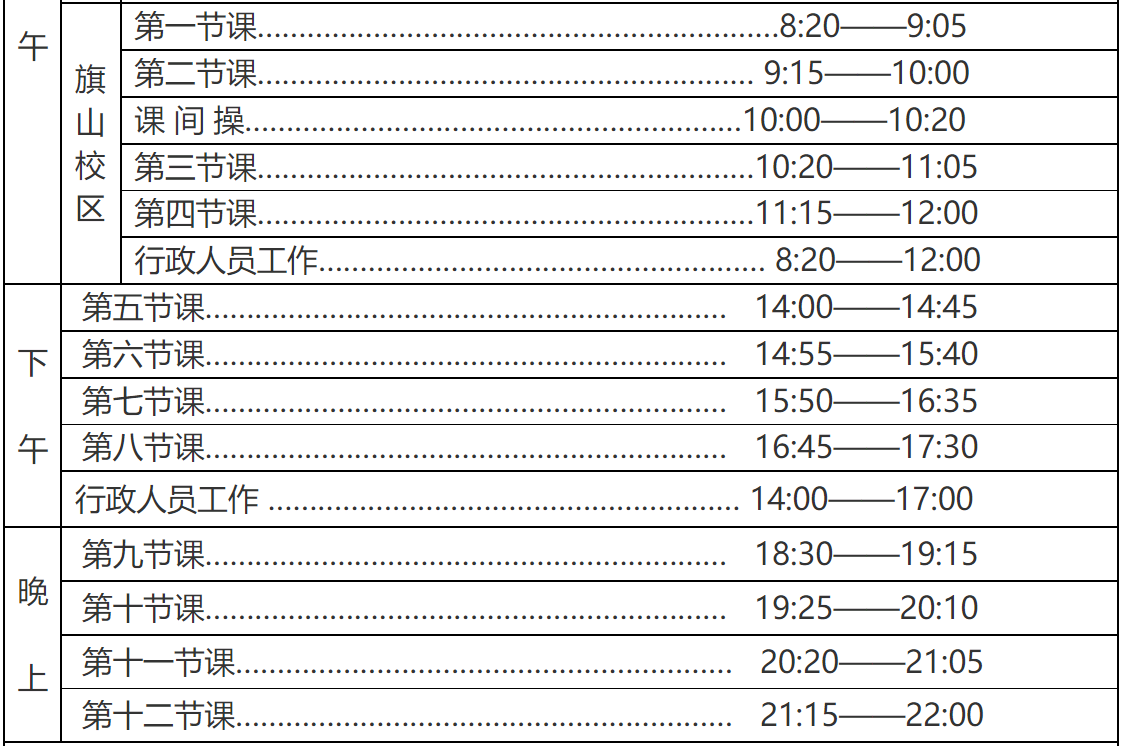
\includegraphics[width=0.9\textwidth]{zx.png}
\end{figure} 

\subsection{附件4:绩点计算方法}

\begin{figure}[H]
	\centering
	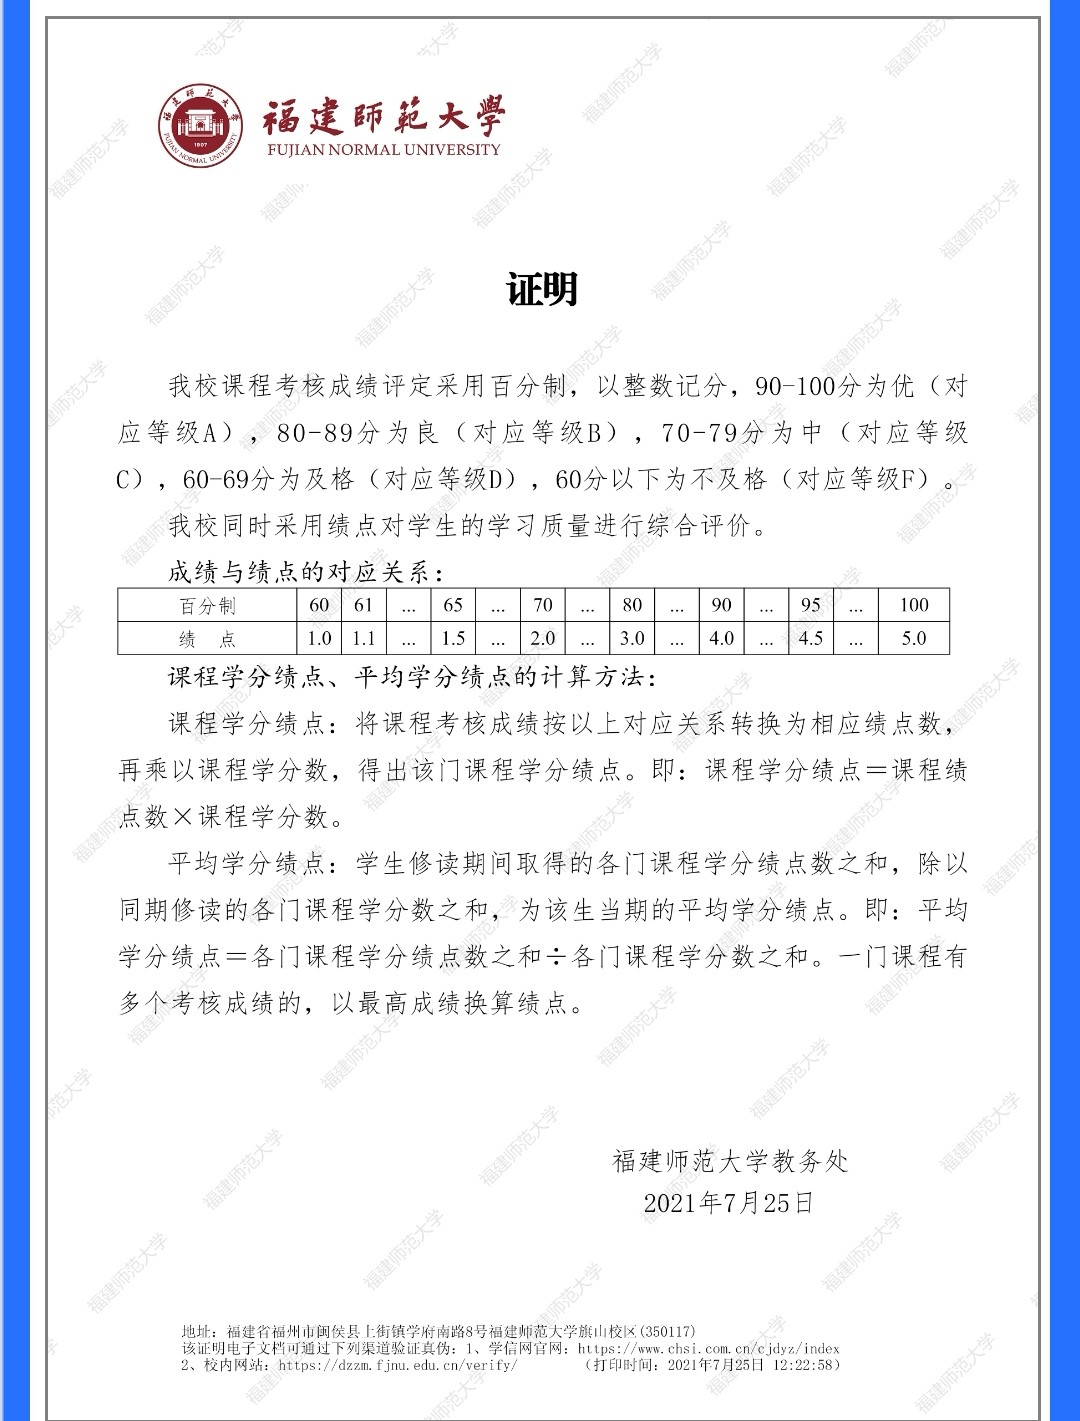
\includegraphics[width=0.9\textwidth]{gpa.jpg}
\end{figure} 

\newpage

\subsection{附件5:数学分析注记}\label{f5}
节选自楼红卫老师的数学分析注记

\begin{figure}[H]
	\centering
	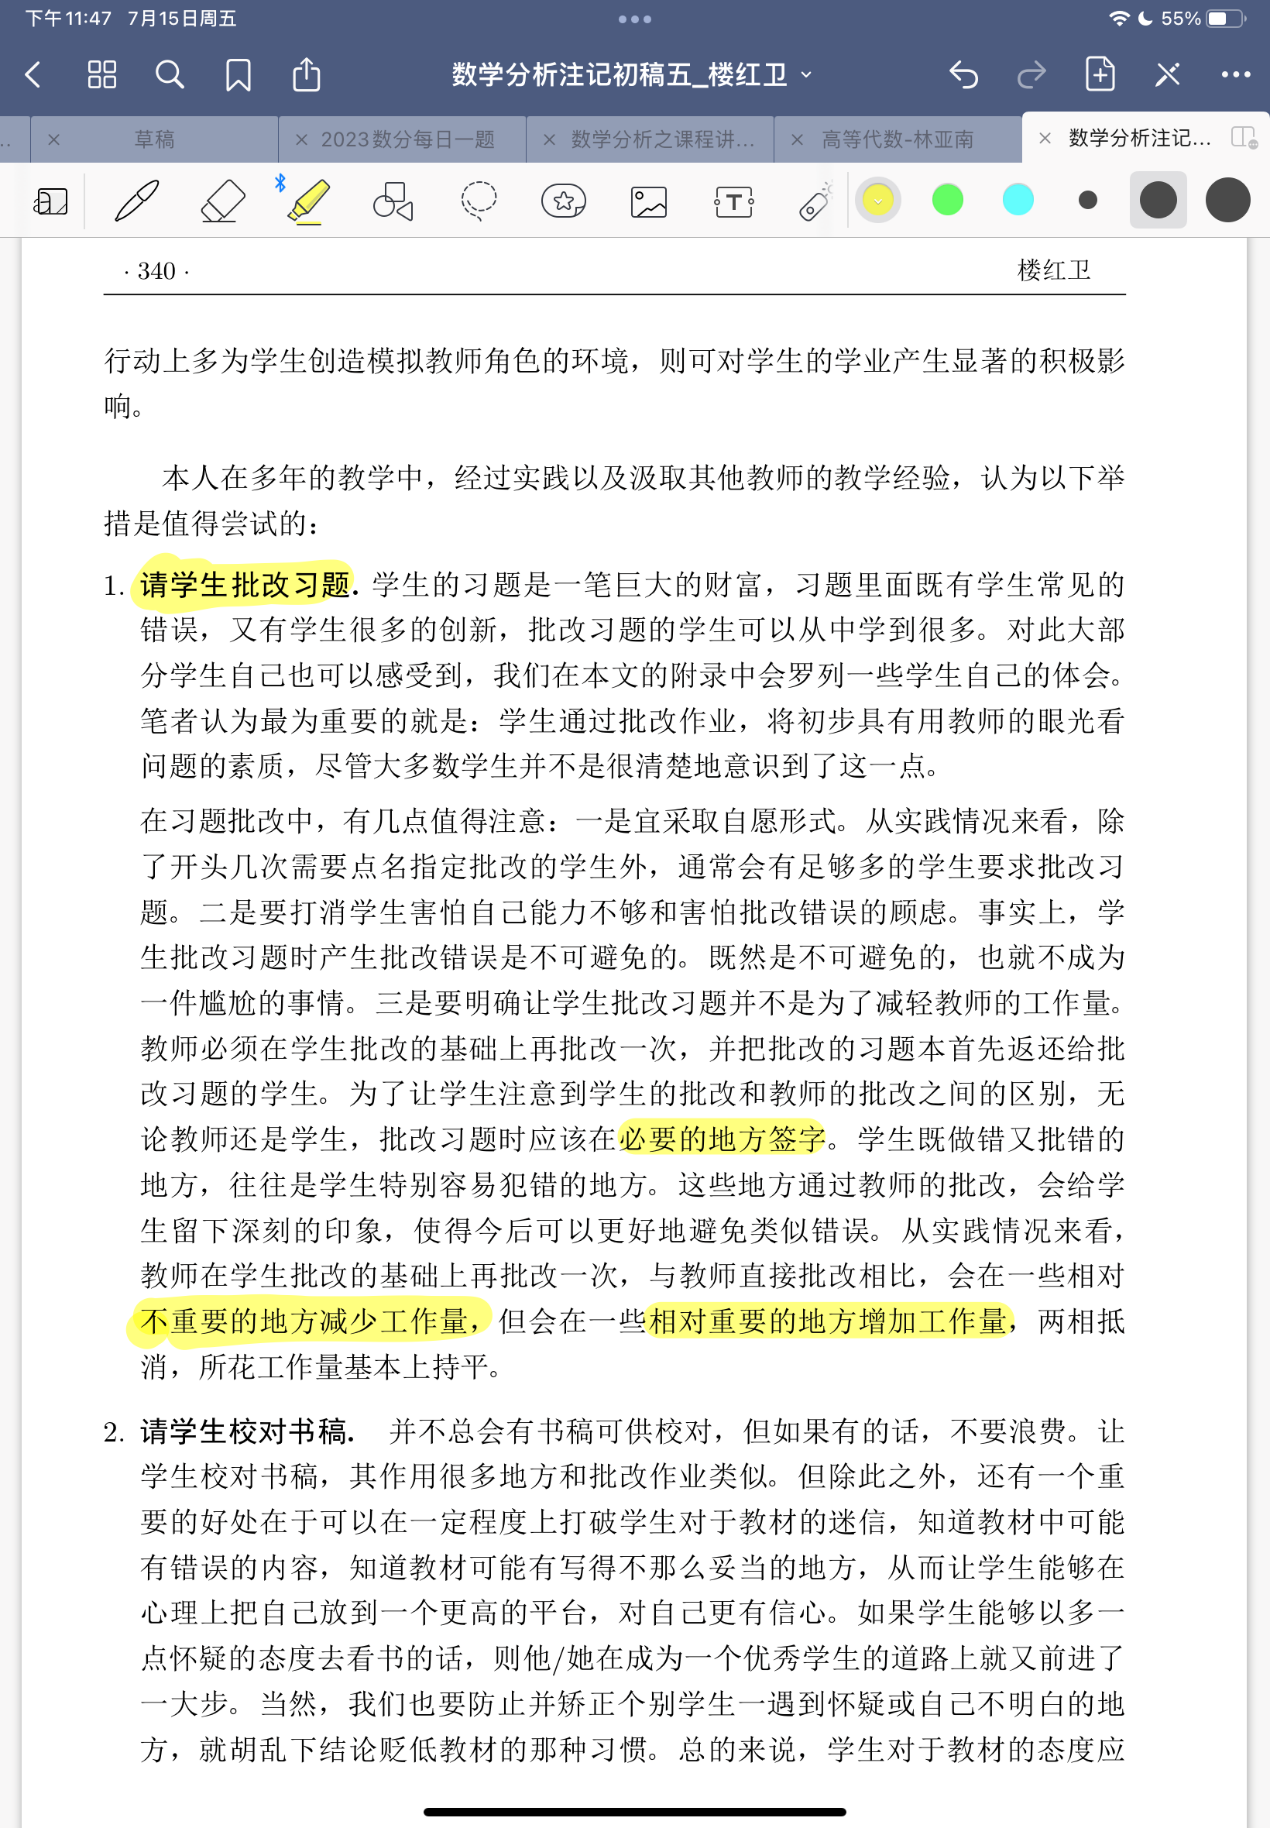
\includegraphics[width=0.9\textwidth]{zhu1.png}
\end{figure} 

\begin{figure}[htbp]
	\centering
	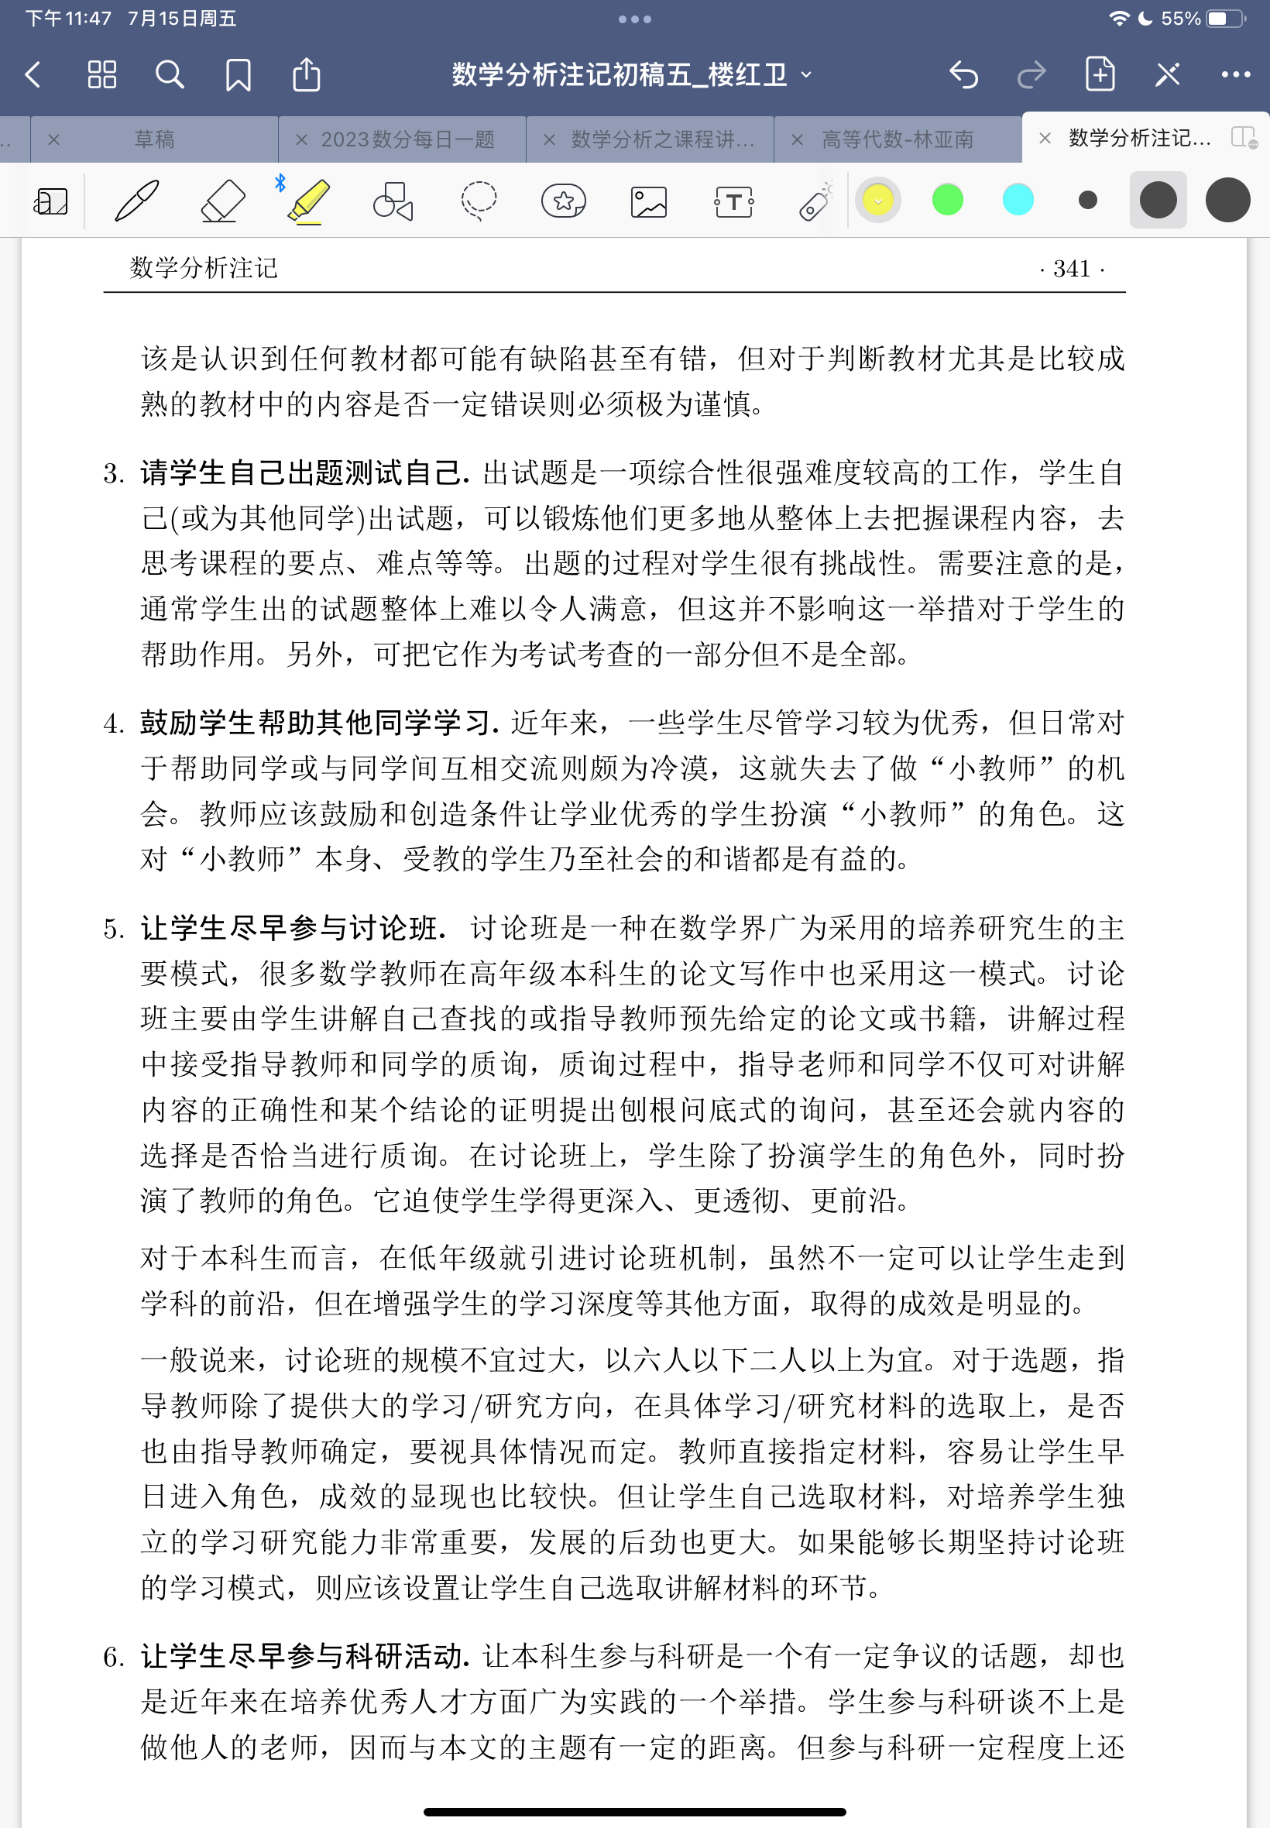
\includegraphics[width=0.9\textwidth]{zhu2.png}
\end{figure} 

\begin{figure}[htbp]
	\centering
	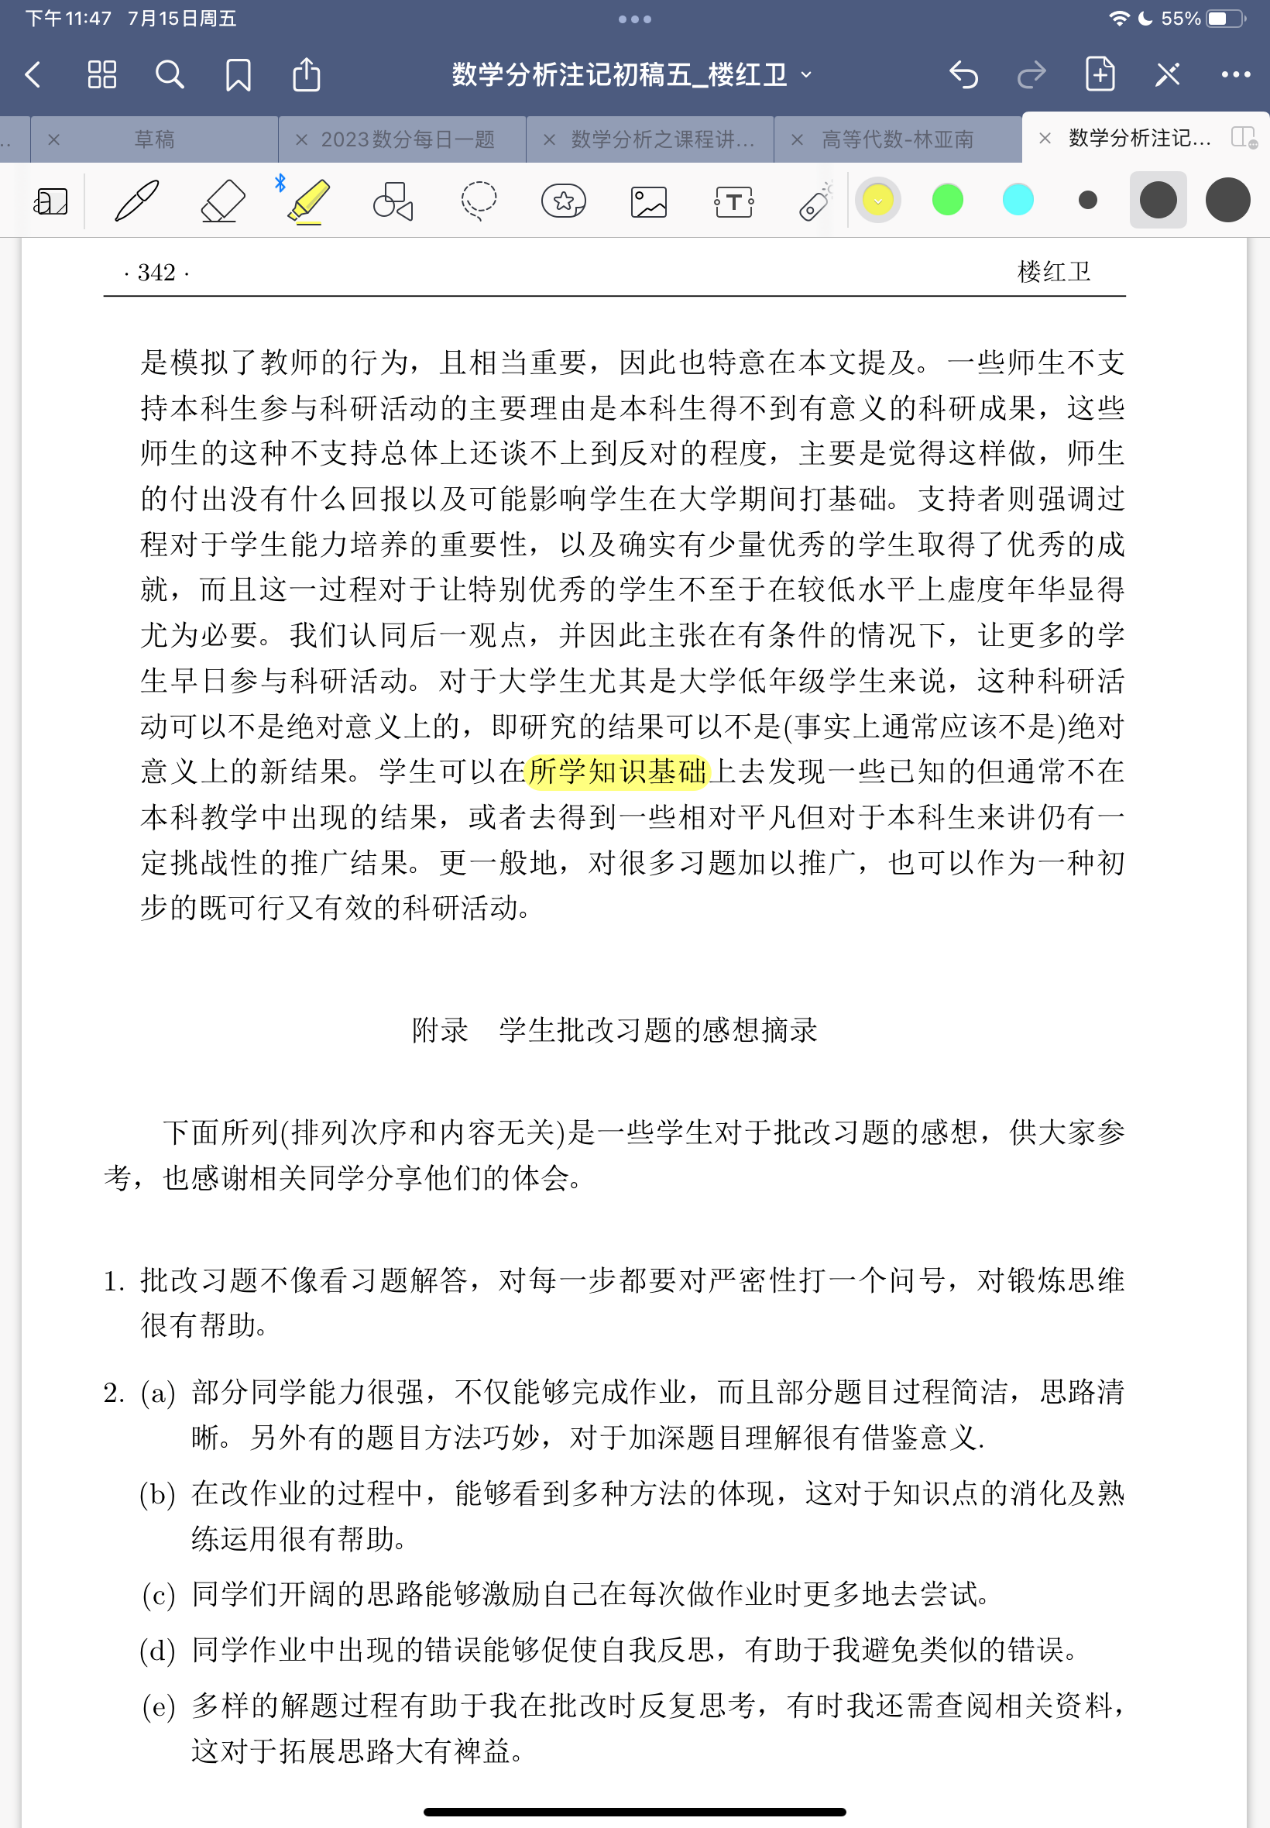
\includegraphics[width=0.9\textwidth]{zhu3.png}
\end{figure} 


\newpage

\section{大一数学类专业课程}\label{sug}
首先要说明,学一门课程可以有很多作为辅助参考作为主教材某部分的\textcolor[rgb]{1,0,0}{拓展},但\textcolor[rgb]{1,0,0}{主教材}(即学校选定)的内容一定要学精通!课后习题保证都做一遍!

\textbf{数学分析主教材:华东师大第五版,高等教育出版社}

\textbf{高等代数主教材:厦门大学林亚南,高等教育出版社}

\textbf{解析几何主教材:福师大自编讲义,尚未出版}

\textbf{以上这几本开学的时候都会发,所以想预习的同学就不要买主教材了。可以先看看电子版(见附件压缩包)。你想预习配套网课看的话,数分陈纪修+高代丘维声即可。}

数分教材参考书:陈纪修的数学分析、史济怀的数学分析教程、梅加强的数学分析第二版

数分习题集:\textcolor[rgb]{1,0,0}{谢惠民}的数学分析习题课讲义作为课本外的补充、裴礼文

高代教材参考书:谢启鸿的高等代数学(也称为绿皮书)、丘维声的高等代数(里面包含习题)、蓝以中的高等代数简明教程(配套学习指南使用)

高代习题集:谢启鸿的高等代数(也称为白皮书)、蓝以中的高等代数学习指南

解析几何参考书:吕林根的解析几何、丘维声的解析几何

\subsection{数学分析}
数学分析其实就是高等数学plus,在微积分里面加上了分析体系,难度跟高数差挺多的。主要关注点在于推理证明上。

上课要认认真真听,做笔记的话不一定要追求将老师板书的每个字都记到,有的时候一直在抄笔记,没有自己的思考效果不是太好。个人建议还是把老师板书的主干记下来,课后自己思考补充,当然课上没想清楚,可以在笔记旁边做个记号。自己对定理建立主观感觉很重要,因此才要举很多例子。

当然有些同学习惯就是先\textcolor[rgb]{1,0,0}{预习}一下,这样确实对你上课大致知道老师会讲什么,帮助比较大。但是有的时候老师不一定会按课本讲的哦,他可能会参考好几本教材混合起来一起讲。所以建议你读书的时候不一定只看一本教材。比如数分1最开始实数的构造有很多种讲法,高进寿老师先前选用的就是Dedekind分割而不是无穷小数法。

数学分析这一门课作为基础课,水还是很深的,很多后续课程研究的原型都起源于这一门课

实验班高进寿老师布置的补充题、上课的内容、深度广度较大。如果没分到数实,你们没课的时候也可以去听听高进寿老师的上课,当然如果你想听别的专业的课也不是不行,课表的话你到教务系统上找推荐课表打印就能找到了,大学听课这一点还是很自由的。

\subsubsection{个人建议}
自己课后有时间的话,去把课本证明自己都推导一遍。想考高分的话,强力推荐精读谢惠民的数学分析习题课讲义,其中很多例题很有启发性,基本上压轴题就是这本里的课后习题或者例题改编。中科大史济怀的数学分析教程课后习题也很不错。

不过说实话,其实如果你跟着高进寿老师,我认为你能把老师每次布置的\textcolor[rgb]{1,0,0}{补充题}认认真真吃透了,有的时候题目做不出来查一查谢惠民、史济怀,再适当额外做一部分习题其实题量就够了,更多的训练可以留到寒暑假,平时课也挺多的。

下面只是介绍一些参考资料:
\begin{enumerate}
    \item 	看网课和看其他教材。网课的资源相比高代而言,没有那么丰富。想看网课的话,可以买一本复旦陈纪修的数学分析,配套b站陈纪修老师的上课视频看;听说B站浙江大学苏德矿老师的微积分课也很不错。个人强烈推荐实数的构造可以看清华刘思齐老师的数学分析1。b站id我真不懂分析。
    \begin{figure}[htbp]
	\centering
	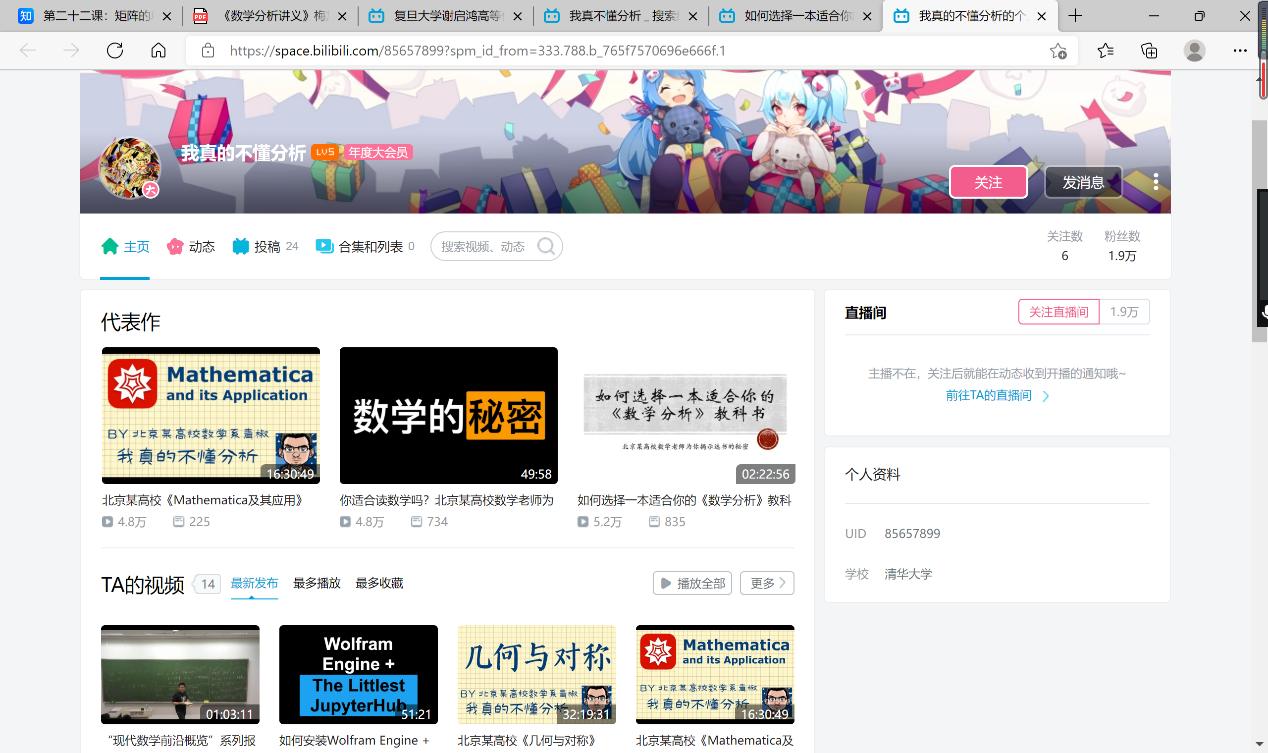
\includegraphics[width=0.75\textwidth]{sf1.png}
\end{figure} 
    \item 	借用刘思齐老师提到的:每个课本都反映作者数学的三观,而你想要认识完整的体系不可能只去学一个人的理解;可以选择1-2本精读(我个人是华师课本+谢惠民的讲义+史济怀)。另外书上有的地方也会出错。可以参考其他课本完善这几本书证明的不足。
    \item 	选书的难度也是因人而异的。我最开始看实数的构造实在理解不了华师课本的讲法。刚开始看史济怀也感到晦涩难懂。建议学完第七章后看史济怀是无障碍的。前6章我看的是复旦陈纪修。数分选书参考这个视频即可。(注:他们选用的教材难度都比较高,视频中提到史济怀不太好这一点可以忽略,数分教材难度是没有上界的。)
        \begin{figure}[H]
	\centering
	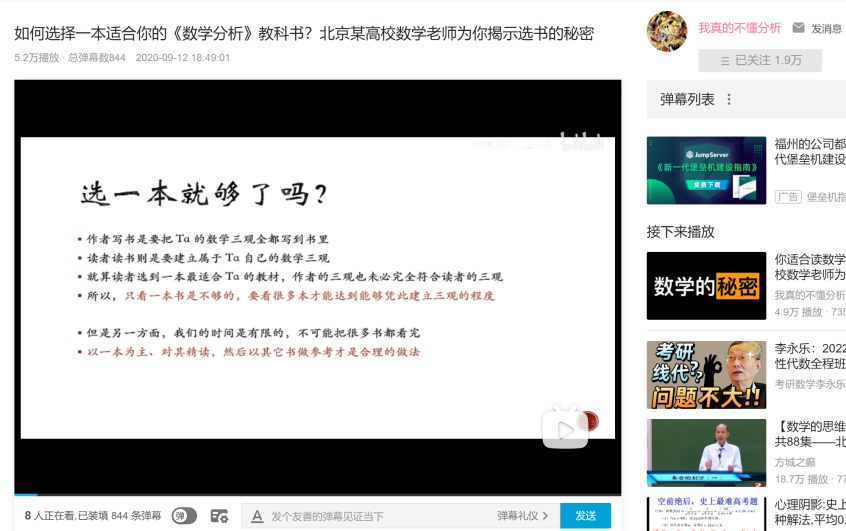
\includegraphics[width=0.75\textwidth]{sf2.png}
\end{figure} 
\end{enumerate}

补充参考书目:红皮北大的数学分析解题指南、张筑生的数学分析新讲(注意一定要配套习题集使用,只看定理不做题等于没学)。

Ps. 20级数实的数分讲授内容:基本是结合中科大的数学分析教程以及习题课讲义的内容讲授的,习题课和小测主要出自习题课讲义。

如果你想学更多,可以试试清华于品数分讲义、卓里奇、rudin、菲赫金哥尔茨等等。因为于品数分讲义习题质量很高,但特别现代,而且一些地方有笔误,你感觉不对的话,可以赶紧去问问助教或者老师。

\subsection{高等代数}
入门:我个人选用的是丘维声,配套b站的上课视频,你可以先买一本上册。

就教材衔接程度来说,个人建议是直接买本复旦大学高等代数学,以及复旦的高代白皮书(涵盖了海量题型),b站上有上课视频以及高等代数习题课。

个人认为厦大高代课后习题给的太少了,不过厦大高代配套学习辅导书编写的题目也很不错。自己找网课的话推荐厦大林亚南以及复旦谢启鸿。两本书下册区别有复旦没有Frobenius标准型、二次型和内积空间顺序的调整,但不影响学习。

复旦高代体系真的已经很完善了,而且谢启鸿老师的网课不但讲了课内知识,有的时候也会补充其他内容。我上课理解不了,一般是多听几遍网课加深印象。

(ps.谢启鸿老师说第四版最快将会在10月与大家见面,我是打算支持一下正版,因为这本书实在写的太好了www)

\subsubsection{个人建议}
\begin{enumerate}
    \item 如果你觉得下面推荐的书太多就看复旦那本就够了,题目解答参考复旦白皮书。如果就针对考试的话厦大课后习题会做,复习题大部分理解就够了。如果自己学一定要保证进度跟老师基本一致,否则你就会陷入以为自己学了很多,实则已经落后别人很多的处境。复旦白皮书上有很多二级结论更适用于考研、竞赛。
    \item 另外一本就是高等代数学习指南,感觉评议写的很好,但是课本简明教程课后习题难度偏大。丘维声老师写的可读性很强,网课也很好。但是你想上课的平时看完他书上所有内容并仔细理解,时间不一定够。建议作为参考。
    \item  节选自高等代数学习指南
    \begin{figure}[H]
	\centering
	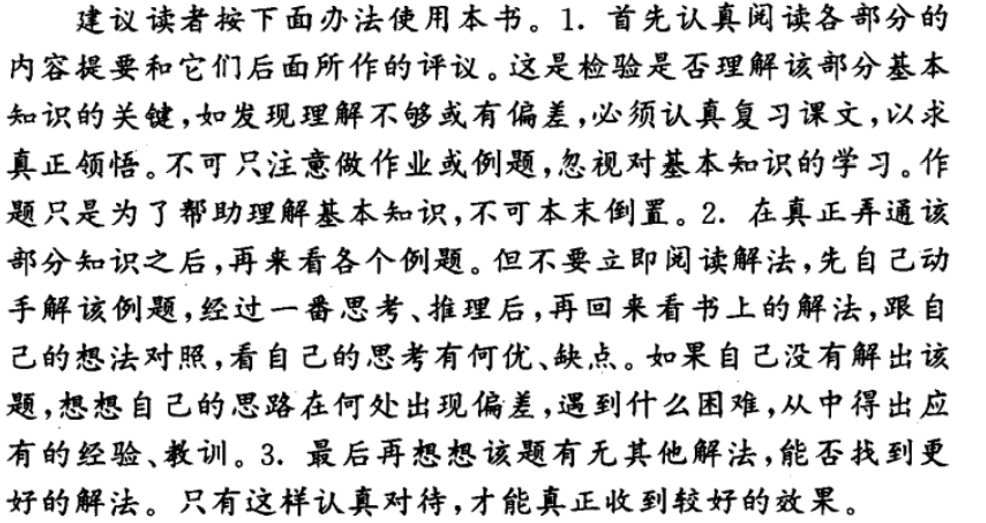
\includegraphics[width=0.9\textwidth]{gd1.png}
    \end{figure} 
    \item 	一定要自己把知识框架能独立写出来。高代同样有很多构造性证明,第一次看到不一定想得到,只能学着去模仿,一般一道题卡10几分钟我会扫一眼答案的关键。可能对我来说,最有效的可能还是像数分讲义一样作一些提示。
    \item   复旦高等代数习题课
    \begin{figure}[H]
	\centering
	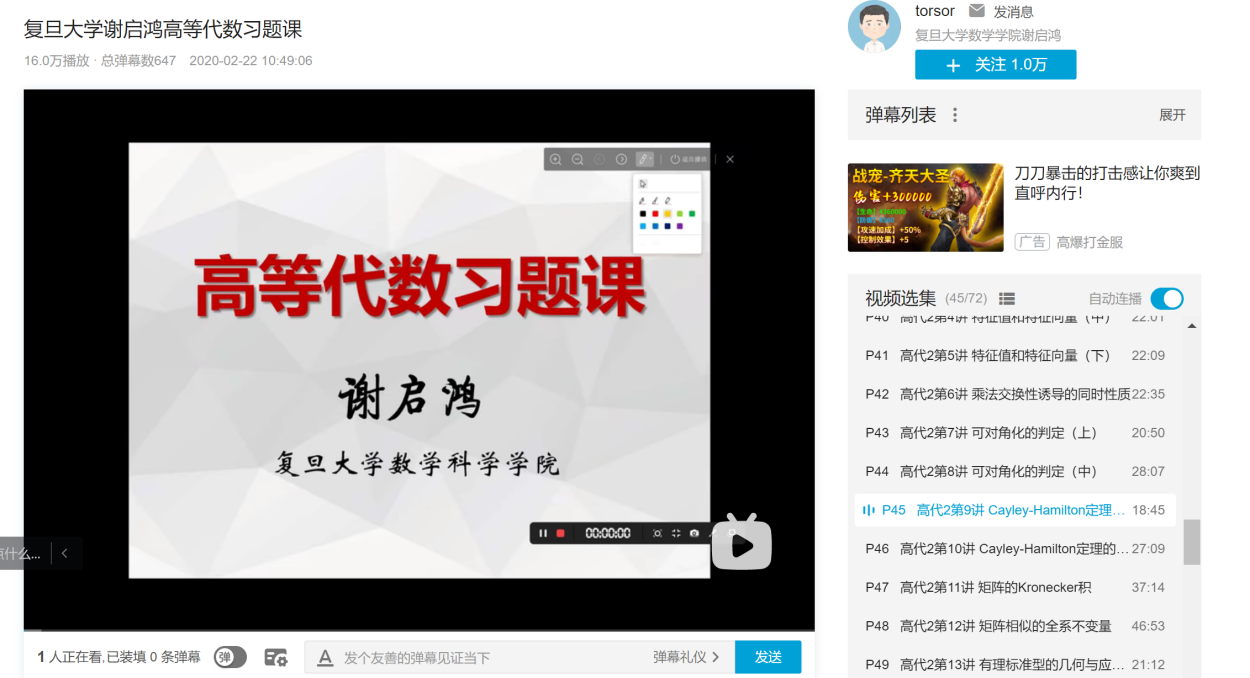
\includegraphics[width=0.9\textwidth]{gd2.png}
    \end{figure} 
\end{enumerate}

想要提高的同学可以参考复旦高代博客的每周一题。

https://www.cnblogs.com/torsor/p/6082082.html


\subsection{解析几何}
相对前两门而言比较简单。就是师大自己编写的课本没有答案(所以老师讲评的时候要认真记,当然也可以找学长学姐看看有没有答案)。

另外,课本上可能部分有印刷错误还没改,自己要注意一下。

题目做不出来看看书上的证明过程,可能会有一定启发性。我当时学的时候经常跟老师的证明想法不大一样,但跟老师讨论之后也是对的。请务必要跟上老师的进度,不然期末会复习的很辛苦。可以买本吕林根、丘维声的解析几何作为参考。

部分高校(比如中科大)考研会考解几,以及在数分三的学习也会用到解几的知识。课程不难并不代表不重要,需引起一定重视。

当然也有清华刘思齐老师的几何与对称这门课,他们是把解析几何换成了这个,但是他们讲的东西也不大一样,前面讲了一些数学史和数理逻辑。闲着没事的时候也可以补一补当知识扩展,我觉得挺好的。

\subsection{大一数学系公共课程介绍}
\subsubsection{大一上}
1. 大学英语(公共必修课,有1234四个学期,每个学期都有。免修申请统一在大一下学期结束,可以免掉大二学年的英语课)

2. 大学体育(公共必修课,一周一节,到时候会有选课,大一上选的课上一个学期,大一下的课上三学期,也就是到大二下)
(ps.听说18级前,大一期末最后两节和大二开学一个月是上游泳课,应该是大二下考;而19级由于疫情没有游泳课,20级大一期末最后两节也没有游泳课,大二自然没有游泳考试,盲猜此后应该不会再有游泳考试了)

3. 思想道德修养与法治(公共必修课,需小组合作在课堂上演讲ppt,无考试)

4. 军事理论(军理,公共必修课,一学期,开卷考)

\subsubsection{大一下}
1. C语言程序设计。可以考计算机二级的C语言替代这门课的成绩,编程,C语言还好吧,有兴趣大一上就可以自学)B站浙江大学翁恺老师的网课很好,CSDN还有配套的习题集也很经典。

2. 大学物理实验(大物实验,公共必修课,十个必做实验,四个选做实验,然后考试,分为平时成绩,实验原理和过程机考和操作,平时成绩内容的话,基本上看好你的实验报告就好,实验报告一定要要弄好,努力拿高分。复习也可以用。操作十个必做实验随意抽一个,考前十分钟会把你要做的实验发群里,操作考也会让你写东西,一般是一些简单的原理和简单的数据处理,后面考的优势较大,因为题目都出来了,可以问别人要写的是什么,数据处理就看你的报告了,所以报告一定要弄好!!!!!大物实验不及格直接重修,没有补考)

3. 大学物理(分为大物上下,大二上学期还要上,公共必修课,据说是从学习通给的资料里面有个清华题库,考前刷一刷清华题库吧,基本就是微积分+高中物理+一些物理知识的拓展。来不及的话就去B站搜峰考物理速成90+)

4. 公共选修课(在大一上学期末选课,第一轮随机筛选与网速无关,第二轮补选拼手速。学校规定每个人必须修满八个公共选修课学分,一门两个学分,另外四门选修课中一定要有一门中外文化与人文素养、一门美育体育与审美体验、一门师德养成与教育法治)

5. 中国近现代史纲要(20级期末闭卷,21级开卷)

6. 大学生心理健康教育(学习通网课刷满,期末考卷多写点)

7.职业生涯规划(期末交篇论文,还好)

\end{document}
